\section{22.03.2018 - Umfrage: Mahout / Recommender}
\begin{itemize}
\item[-] Fragen Sie Ihre Kommilitonen nach Filmen, Getränken, Büchern, Musikvorlieben, etc.
\item[-] Lassen Sie obiges bewerten (1 bis 5 Sterne).
\item[-] Analysieren Sie die Umfrage mit Mahout Recommender
\end{itemize}

\subsection*{Kurzdarstellung der Aufgabenstellung}
Es soll eine Bewertungsumfrage bzgl. Büchern, Film o.Ä. getätigt werden. Hierbei sollen die Teilnehmer die jeweiligen Titel mit 1 bis 5 Sternen bewerten. Es ist hierbei von kritischer Bedeutung das kein Teilnehmer alle Titel/Objekt der Umfrage bewertet.

Die gesammelten Daten müssen entsprechend in Form einer .csv Datei aufbereitet werden für das anschließende Importieren in die Software. Nach dem Einlesen werden für einige Umfrageteilnehmer x Empfehlungen mit höchster Gefallenswahrscheinlichkeit abgefragt (abgeleitet aus den Bewertungen anderer Teilnehmer).

\subsection*{Lösung}
\begin{itemize}
\item[-] Visualisierung der getätigten Umfrage von 10 Teilnehmern zu 17 verschiedenen Filmen (\autoref{fig:recommender1}):
\begin{figure}[!htb]
        \begin{minipage}{1\textwidth}
                \centering
                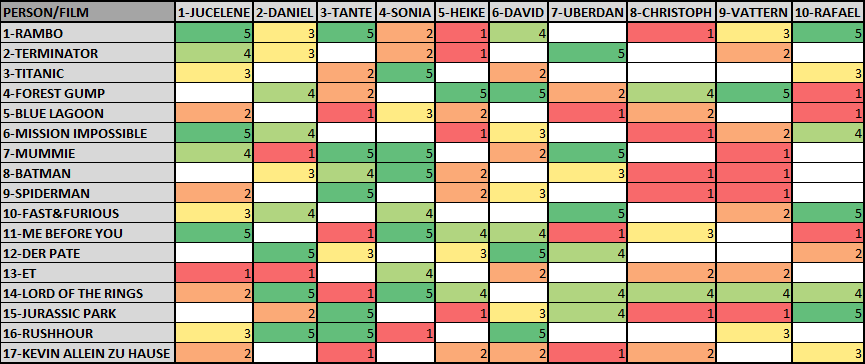
\includegraphics[width=0.90\textwidth]{pics/recommender1.png}\par\vspace{0cm}
                \caption{Tabelle: Umfrage}
                \label{fig:recommender1}
        \end{minipage}
\end{figure}

\item[-] Aufarbeitung Umfrage mit Excel für vorgegebenes Format: userID, itemId und prefValue (\autoref{fig:recommender2})
\begin{figure}[!htb]
        \begin{minipage}{1\textwidth}
                \centering
                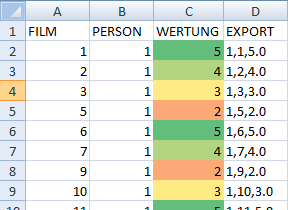
\includegraphics[width=0.90\textwidth]{pics/recommender2.png}\par\vspace{0cm}
                \caption{Tabelle: Aufarbeitung der Umfrage}
                \label{fig:recommender2}
        \end{minipage}
\end{figure}

Starten Oracle 4.9 VM

\item[-] Kopieren der Daten aus Spalte D in die Datei namen „dataset.csv“ Ordner /usr/temp/

\item[-] Oracle Jdeveloper starten

\item[-] Neues Java project angelegt: „myproject“ (gleicher Pfad Projekt)

\item[-] Bibliotheken aus den folgenden Ordnern hinzugefügt:
usr/lib/hadoop (all Library),
usr/lib/hadoop/lib (all Library),
usr/lib/Mahout/ (all Library),
usr/lib/Mahout/lib (all Library)

\item[-] Inhalt der recommender.txt Datei vom ELLI in das Java Projekt kopieren und den Filedatamodel und für die Emfpehlungsabfrage entsprechend die gewünschte Userid und Anzahl von Empfehlungen aufführen:
\end{itemize}

\begin{enumerate}
\item User 1 sollen nun 2 Filme empfohlen werden was zum Ergebnis in \autoref{fig:recommender3} führt:
\begin{figure}[!htb]
        \begin{minipage}{1\textwidth}
                \centering
                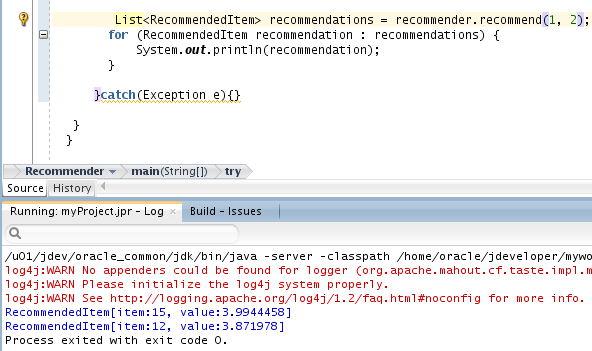
\includegraphics[width=0.90\textwidth]{pics/recommender3.png}\par\vspace{0cm}
                \caption{Tabelle: Ergebnis für User1}
                \label{fig:recommender3}
        \end{minipage}
\end{figure}

Es werden mit einer „Wahrscheinlichkeit des Gefallens“ von 3,87/5 bzw. 3,99/5   Userid 1 die Filme 12 („Der Pate“) und 15 („Jurassic Park“) empfohlen. Was augenscheinlich plausibel ist.

\item User 2 sollen nun 2 Filme empfohlen werden was zum Ergebnis in \autoref{fig:recommender4} führt:
\begin{figure}[!htb]
        \begin{minipage}{1\textwidth}
                \centering
                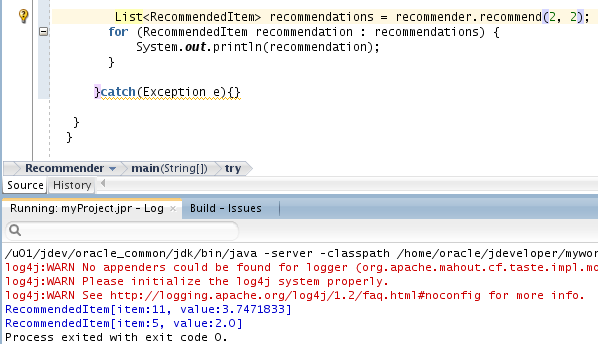
\includegraphics[width=0.90\textwidth]{pics/recommender4.png}\par\vspace{0cm}
                \caption{Tabelle: Ergebnis für User2}
                \label{fig:recommender4}
        \end{minipage}
\end{figure}

Es werden mit einer „Wahrscheinlichkeit des Gefallens“ von 3,75/5 bzw. 2/5 Userid 2 die Filme 11 („Me before You“) und 5 („Blue Lagoon“) empfohlen. Was augenscheinlich plausibel ist.

\item User 3 sollen nun 2 Filme empfohlen werden was zum Ergebnis in \autoref{fig:recommender5} führt:
\begin{figure}[!htb]
        \begin{minipage}{1\textwidth}
                \centering
                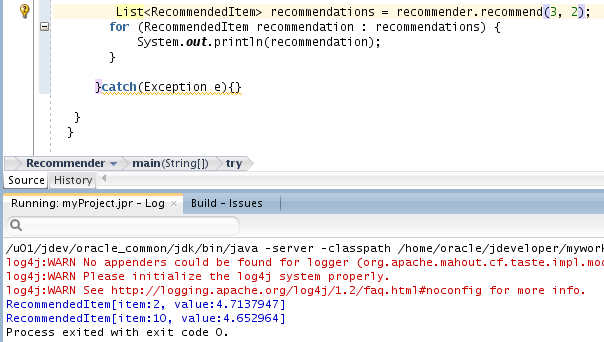
\includegraphics[width=0.90\textwidth]{pics/recommender5.png}\par\vspace{0cm}
                \caption{Tabelle: Ergebnis für User3}
                \label{fig:recommender5}
        \end{minipage}
\end{figure}


Es werden mit einer ''Wahrscheinlichkeit des Gefallens`` von 4,71/5 bzw. 4,65/5 Userid 2 die Filme 10 (``Me before You``) und 5 (``Fast \& Furious``) empfohlen. Was augenscheinlich plausibel ist.

\end{enumerate}

\subsection*{Aufteilung der Aufgaben im Team}
\subsection*{Darstellung der benutzen Werkzeuge und Systeme}
\subsubsection*{Entwurfswerkzeug}
Microsoft Excel
\subsubsection*{Entwicklungsumgebung}
JDeveloper

